%%%%%%%%%%%%%%%%%%%%%%%%%%%%%%%%%%%%%%%%%%%%%%%%
\input{./format/preamble.ltx} 

%%%%%%%%%%%%%%%%%%%%%%%%%%%%%%%%%%%%%%%%%%%%%%%%
% as needed, comment the following lines by prefixing the percent sign at the start of the line

%\PutLineNumberstrue % comment to disable line numbers and certain  preparation guides 

\Figurestrue % comment to disable the rendering figures

%\GroupIDtrue % comment to disable group ID

%\ResultDiscusstrue % comment to disable results and discussions

%\Conctrue % comment to disable conclusions

%\Finishedtrue % comment to disable manuscript for final hard binding

%\Gradtrue % comment to disable graduate school format

%\PhDtrue % comment to disable PhD dissertation format

%\PubListtrue % comment to disable publication list

%\Vitatrue % comment to disable author(s) vita

%\Indextrue % comment to disable index 

%%%%%%%%%%%%%%%%%%%%%%%%%%%%%%%%%%%%%%%%%%%%%%%%
% document IDs

% specify if dissertation, thesis, project, dissertation proposal, thesis proposal, project proposal 
\newcommand{\documentType}{Thesis} 
%\newcommand{\documentType}{Thesis Proposal}
%\newcommand{\documentType}{Dissertation Proposal}
%\newcommand{\documentType}{Dissertation}
\newcommand{\college}{Gokongwei College of Engineering}
\newcommand{\department}{Department of Electronics and Communications Engineering} 
\newcommand{\degreeType}{Bachelor of Science}
%\newcommand{\degreeType}{Bachelor and Master of Science}  
%\newcommand{\degreeType}{Master of Engineering Program} 
%\newcommand{\degreeType}{Master of Science} 
%\newcommand{\degreeType}{Doctor of Philosophy} 
\newcommand{\degree}{Electronics and Communications Engineering}
\newcommand{\degreeAbbrv}{BS-ECE}
%\newcommand{\degreeAbbrv}{BS-MS-ECE}
%\newcommand{\degreeAbbrv}{MEP-ECE}
%\newcommand{\degreeAbbrv}{MS-ECE}
%\newcommand{\degreeAbbrv}{PhD-ECE}

\newcommand{\documentAdviserTitle}{Engr.} 
\newcommand{\documentAdviser}{Maria Antonette C. Roque}

\newcommand{\examinerChairTitle}{Dr.} 
\newcommand{\examinerChair}{Amado Z. Hernandez}

% Sort in alphabetically ascending manner the surnames of the examiners
\newcommand{\examinerATitle}{Dr.} 
\newcommand{\examinerA}{Jose Y. Alonzo}

\newcommand{\examinerBTitle}{Dr.} 
\newcommand{\examinerB}{Mariana X. Mercado}

% Note that \examinerC and \examinerD only applies for PhD dissertations
\newcommand{\examinerCTitle}{Dr.} 
\newcommand{\examinerC}{Rafael W. Sison}

\newcommand{\examinerDTitle}{Dr.} 
\newcommand{\examinerD}{Apolinario V. Valenzuela}

\newcommand{\deanTitle}{Dr.} 
\newcommand{\deanName}{Diego U. Lopez}

\newcommand{\groupID}{ESG-04} % group ID is for undergraduates as of this formatting

\newcommand{\numberOfAuthors}{4} % adapt the number of names below accordingly and sort the sunames in alphabetically ascending manner, like in the following example

\defineAuthor{surname1}{Guevarra}
\defineAuthor{firstname1}{Alnair M.}

\defineAuthor{surname2}{Hernandez}
\defineAuthor{firstname2}{Roy Stephen A.}

\defineAuthor{surname3}{Lagman}
\defineAuthor{firstname3}{Maria Josefa M.}

\defineAuthor{surname4}{Villanueva}
\defineAuthor{firstname4}{Andre Micayle P.}

\defineAuthor{surname5}{Rianzares}
\defineAuthor{firstname5}{Max V.}

\newcommand{\documentTitle}{Driver Fatigue Detection Using an RGB-D Sensor Based On Eye Tracking and Head Pose Estimation} % put tilde (~) between words to indicate non-breaking adjacent words

\newcommand{\keywords}{Eye Tracking, RGBD camera, MyRio}

\newcommand{\approvalDate}{\usdate\today} % put here the date when all examiners have given their approval; do not remove the tildes in order to not break the date; the submission deadline can also be placed as the date

\hyphenation{op-tical net-works semi-conduc-tor evi-dent re-la-tive re-si-den-tial po-la-ri-za-tion so-lu-tion/s} % for correcting bad hyphenation

%%%%%%%%%%%%%%%%%%%%%%%%%%%%%%%%%%%%%%%%%%%%%%%%
\input{./format/postamble.ltx} 

%%%%%%%%%%%%%%%%%%%%%%%%%%%%%%%%%%%%%%%%%%%%%%%%
% for placing user-defined-ambles

\DeclareMathAlphabet{\mathitbf}{OML}{cmm}{b}{it} %for math italic bold 

%%%%%%%%%%%%%%%%%%%%%%%%%%%%%%%%%%%%%%%%%%%%%%%%
% \includeonly{} is for specifying which files to include; if you only want to work on one or few chapters, you can only include those chapters, which will speed up the document build; advantage: fast if you have a large number of images in your results chapter, which you do not need when you are working on other chapters; you can still reference all the figures in the omitted chapter, as long as you have previously LaTeX-built the entire document

% Note that the file names below must correspond to those names inside \include{} in the \begin{document} ... \end{doument} enviroment, otherwise the chapter will not be included

%  the excludeonly package provides the logically opposite command: \excludeonly{<file list>}

\includeonly{% just comment those portions that you do not want to be included in the parsing
introduction,
literature_review,
%theoretical_considerations,
%design_considerations,
%methodology,
%results_and_discussion,
%conclusions,
%answers_to_questions,
%usage_examples,
%publication,
%vita,
}

%%%%%%%%%%%%%%%%%%%%%%%%%%%%%%%%%%%%%%%%%%%%%%%%
\begin{document}
\pagenumbering{roman} % roman page numbering starts here

%%%%%%%%%%%%%%%%%%%%%%%%%%%%%%%%%%%%%%%%%%%%%%%%
\input{./format/pre_toc.ltx}
\cleardoublepage

%%%%%%%%%%%%%%%%%%%%%%%%%%%%%%%%%%%%%%%%%%%%%%%%
\begin{SingleSpace}
\tableofcontents
\cleardoublepage

%%%%%%%%%%%%%%%%%%%%%%%%%%%%%%%%%%%%%%%%%%%%%%%%
\listoffigures
\cleardoublepage

%%%%%%%%%%%%%%%%%%%%%%%%%%%%%%%%%%%%%%%%%%%%%%%%
\listoftables
\cleardoublepage

%%%%%%%%%%%%%%%%%%%%%%%%%%%%%%%%%%%%%%%%%%%%%%%
\begin{comment}
\phantomsection
\addcontentsline{toc}{chapter}{Abbreviations}
{
	\printterms[database=abbreviation, style=indexalign, prelocation=dotfill, location=first, columns=1, postname=\hspace{3em}]
	\thispagestyle{plain}
}	
\cleardoublepage
\end{comment}
%%%%%%%%%%%%%%%%%%%%%%%%%%%%%%%%%%%%%%%%%%%%%%%
\begin{comment}
\phantomsection
\addcontentsline{toc}{chapter}{Notation}
{
	\printterms[database=notation, style=indexalign, prelocation=dotfill, location=first, columns=1, postname=\hspace{3em}]
	{
	\vspace{3ex}
	\noindent Throughout this \MakeTextLowercase{\documentType}, mathematical notations conform to ISO~80000-2 standard, e.g. variable names are printed in italics, the only exception being acronyms like e.g. $\mathrm{SNR}$, which are printed in regular font.  Constants are also set in regular font like $\mathrm{j}$.  Functions are also set in regular font, e.g. in $\sin \left( \cdot \right)$.  Commonly used notations are $t$, $f$, $\mathrm{j} = \sqrt{-1}$, $n$ and $\exp \left( \cdot \right)$, which refer to the time variable, frequency variable, imaginary unit, $n$th variable, and exponential function, respectively.
	}
	\thispagestyle{plain}
}
\cleardoublepage
\end{comment}
%%%%%%%%%%%%%%%%%%%%%%%%%%%%%%%%%%%%%%%%%%%%%%%%
\begin{comment}
\phantomsection
\addcontentsline{toc}{chapter}{Glossary}
{
	\printterms[database=glossary, style=indexalign, prelocation=none, location=hide, columns=1, postname=\hspace{3em}]
	\thispagestyle{plain}
}
\cleardoublepage
\end{comment}
%%%%%%%%%%%%%%%%%%%%%%%%%%%%%%%%%%%%%%%%%%%%%%%%
%\lstlistoflistings
\cleardoublepage
\end{SingleSpace}

%%%%%%%%%%%%%%%%%%%%%%%%%%%%%%%%%%%%%%%%%%%%%%%%
\pagenumbering{arabic} % arabic page numbering starts here
\chapter{Introduction}
\label{ch:intro}
\startcontents[chapters]
\begin{SingleSpace}	
	\Mprintcontents  % for creating an actual mini TOC for this chapter
\end{SingleSpace}
\section{Background of the Study}

Aside from the usual text descriptions of the background, put here figures that will cast images to your audience about the context of your work.

\textcolor[rgb]{0.75,0.75,0.75}{\Blindtext}


\section{Prior Studies}

Put here a \index{summary}summary of your literature review.  Preferably, a table showing the summary would be helpful. 

Prior Studies or Literature Review (expansion of the Prior Studies) is basically about competition. Competition.

So the goals are:

\begin{enumerate}
	\item to mention briefly the problem; 

	\item to show the features of the existing literature in solving the problem

	\item to show the weakness of the solutions of existing literature 

	\item to show how your solution is better (can be better (for proposals))
\end{enumerate}

\noindent For the table that is placed here, please discuss it in light of the above-mentioned goals. The main difference between the Prior Studies and Literature Review is that the Prior Studies is done in a concise manner.

 \textcolor[rgb]{0.75,0.75,0.75}{\blindtext}


\section{Problem Statement}

The problem statement needs to be very clear and to the point. 

\noindent A persuasive problem statement from a contextualized and intended-audience-awareness perspective consists of:

\begin{enumerate}
	\item PS1: description of the ideal scenario for your intended audience	
	\begin{itemize}
		\item Describe the goals, desired state, or the values that your audience considers important and that are relevant to the problem.
	\end{itemize}
	
	\item PS2:  reality of the situation
	\begin{itemize}
			\item Describe a condition that prevents the goal, state, or value discussed in PS1 from being achieved or realized at the present time.
			\item It is imperative to make the audience feel the pain point.
	\end{itemize}
	
	\item PS3:  consequences for the audience		
	\begin{itemize}
			\item Using specific details, show how the situation contains little promise of improvement unless something is done.
	\end{itemize}

\end{enumerate}

\noindent After the above-mentioned items, succinctly describe your approach/solution ("approach" for proposal theses; "solution" for ``final'' theses). You must be terse here because your approach/solution is like a seed/kernel in terms of its description here, which you expand more through your objectives, and it grows larger in your description and methodology, and its full explanation in the Methodology chapter.

\noindent A well constructed problem statement will convince your audience that the problem is real and worth having you solve it.



\textcolor[rgb]{0.75,0.75,0.75}{\blindtext}



\section{Objectives}

Your objectives are the states that you desire to achieve in solving the problem. The general objective is the main state to be achieved whereas the specific ones are sub-states to be achieved.

\subsection{General Objective(s)}
To \ldots;

\subsection{Specific Objectives}

\begin{enumerate}
	\item To  \ldots;
	
	\item To  \ldots;
	
	\item To  \ldots;
	
	\item To  \ldots;
	
	\item To  \ldots;
\end{enumerate}



\section{Significance of the Study}

\textcolor[rgb]{0.75,0.75,0.75}{\blindtext}



\section{Assumptions, Scope and Delimitations}

Bulletize your assumptions in one group, and then bulletize the scope in another, and do the same for your delimitations.

\subsection{Assumptions}
\begin{enumerate}
	\item \ldots;
	
	\item \ldots;
	
	\item \ldots;	
\end{enumerate}

\subsection{Scope}
\begin{enumerate}
	\item \ldots;
	
	\item \ldots;
	
	\item \ldots;	
\end{enumerate}

\subsection{Delimitations}
\begin{enumerate}
	\item \ldots;
	
	\item \ldots;
	
	\item \ldots;	
\end{enumerate}

\section{Description and Methodology}

A purpose of the description here is to re-steer/remind the panelist/reader again by tersely describing what your thesis is about (i.e. its problem and the main goal you want to achieve). Your methodology is your means of achieving your stated objectives.

Note that each stated objective should have a corresponding methodology.

\textcolor[rgb]{0.75,0.75,0.75}{\blindtext}


\ifFinished
\else

\section{Estimated Work Schedule and Budget}

Gantt chart or project network diagram is to be part of this section.

\textcolor[rgb]{0.75,0.75,0.75}{\blindtext}

\ifPhD
\section{Publication Plan}
\textcolor[rgb]{0.75,0.75,0.75}{\blindtext}
\fi

\fi


\section{Overview}

Provide here a brief summary and what the reader should expect from each succeeding chapter.  Show how each chapter is connected with each other.


\stopcontents[chapters]
\cleardoublepage

%%%%%%%%%%%%%%%%%%%%%%%%%%%%%%%%%%%%%%%%%%%%%%%%
\chapter{Literature Review} 
\label{ch:litrev} 
\startcontents[chapters]
\begin{SingleSpace}	
	\Mprintcontents 
\end{SingleSpace}
It is to be noted that each subsection in this chapter should discuss in narrative form each table that is presented.  

\section{Existing Work}

Cite and summarize here relevant and significant literature (dissertations, theses, journals, patents, notable conference papers) through a table and descriptions to prove that no one has done your work yet and/or that your work is not a duplication of existing ones. Your focus here is what has \emph{been done}.

\graytx{\Blindtext}

\section{Lacking in the Approaches}

You can summarize the weaknesses of existing approaches by a tabular comparison of the literature. Your focus here is what has \emph{not been done}, i.e. what features were missed, what solutions were not considered, what the demerits are, etc.  Through these items, you then can introduce the necessity for doing your proposed solution.  

It is to be noted that degree of novelty for undergraduate thesis is lower than those for graduate school. If a PhD dissertation/thesis has a high degree of novelty and that for an undergraduate is low, then a master's thesis is somewhere between the two.

Briefly include here the following in order to remind the reader why you are highlighting the weaknesses of the solutions of existing literature. 

\begin{itemize}
	\item mentioning of the problem
	\item showing how your solution is better (can be better (for proposals))
\end{itemize}


\graytx{\Blindtext}

\section{Summary}

Provide the gist of this chapter such that it reflects the contents and the message.





\stopcontents[chapters]
\cleardoublepage

%%%%%%%%%%%%%%%%%%%%%%%%%%%%%%%%%%%%%%%%%%%%%%%%
\begin{comment}
\chapter{Theoretical Considerations}
%\chaptermark{Theoretical Considerations} % uncomment this and put a shorter version of the chapter title for the TOC and chapter markings (i.e., header or footer)
\label{ch:theorycon}
\startcontents[chapters]
\begin{SingleSpace}	
	\Mprintcontents 
\end{SingleSpace}
Before starting the first section, provide an overview of the purpose of this chapter and its contents, and how they are relevant to your methodology.  Discuss in this chapter the relevant theories and concepts that should support your proposed solutions.

This chapter is for providing the context to your panelist/reader.  It is actually an expanded form of the Background of the Study that you have put in Chapter~\ref{ch:intro}.

\graytx{\Blindtext}

\begin{figure}[!htbp]
	\centering
		
\includegraphics[width=0.5\textwidth]{example_gray_box}
	\caption{A quadrilateral image example.}
	\label{fig:exampletc}
\end{figure}

\section{Summary}

Provide the gist of this chapter such that it reflects the contents and the message.
\stopcontents[chapters]
\cleardoublepage
\end{comment}
%%%%%%%%%%%%%%%%%%%%%%%%%%%%%%%%%%%%%%%%%%%%%%%%
\begin{comment}
%\chapter{Design Considerations} 
\label{ch:designcon} 
\startcontents[chapters]
\begin{SingleSpace}	
	\Mprintcontents 
\end{SingleSpace}
Before starting the first section, provide an overview of the purpose of this chapter and its contents, and how they are relevant to your methodology. 

Your primary goal in the Design Considerations chapter is to describe to your panelist/readers the key topics that fall further under Theoretical Considerations, but should be placed here instead since they are geared towards your Methodology. These key topics are those that you have directly adopted in making your solution/methodology.  You can think of the connection of the Design Considerations chapter to the Theoretical Considerations chapter in this way: if your Theoretical Considerations chapter serves as the main foundation of a building, then the Design Considerations chapter functions as the columns. 

The  Design Considerations chapter is an avenue for explaining why you considered the topics here for your proposed methodology. This chapter is different from your methodology, because topics you discuss here are already accepted as part of the body of knowledge, and may have not been developed by you.  


\graytx{\Blindtext}


\section{Summary}

Provide the gist of this chapter such that it reflects the contents and message.
\stopcontents[chapters]
\cleardoublepage
\end{comment}

%%%%%%%%%%%%%%%%%%%%%%%%%%%%%%%%%%%%%%%%%%%%%%%%
\begin{comment}
\chapter{Methodology} 
\label{ch:method} 
\startcontents[chapters]
\begin{SingleSpace}	
	\Mprintcontents 
\end{SingleSpace}
Mention here your methodology flow through a figure (preferably) and provide an overview of it and how your methodology achieves your objectives.  How your methodology achieves each of your specific objective is what your panelists/examiners will be looking for. 
Also make sure that you refer clearly to the chapters on the Literature Review, Theoretical Considerations, and Design Considerations showing how your methodology ties with those that you have discussed in those chapters.


\section{Implementation}

Summarize the process used to create/set-up the work with an explanation of such process, instruments, and materials that you used if any. If the description is lengthy, use condensed bullet points. 

\noindent \textit{Rule of thumb}: Implementation is how you made your  work; (keywords: implemented, created, made, soldered, programmed, etc.).

If you wrote a program or made a simulation, you must state how the program or simulation functions in this section.	An algorithm or a pseudocode as shown in Table~\ref{tab:calcxn} is a good example.


\textcolor[rgb]{0.75,0.75,0.75}{\Blindtext}



\section{Evaluation}

Describe the procedures for evaluating the correct behavior and outcome of your  work, including what information you need to gather and how you will obtain or measure it.  

\textit{Rule of thumb}: Evaluation is how you tested your  work; (keywords: measured, tested, compared, simulated, etc.).

\textcolor[rgb]{0.75,0.75,0.75}{\Blindtext}



\section{Summary}

\stopcontents[chapters]
\cleardoublepage
\end{comment}

%%%%%%%%%%%%%%%%%%%%%%%%%%%%%%%%%%%%%%%%%%%%%%%%

\ifResultDiscuss 
	\chapter{Results and Discussion} 
	\label{ch:result_discuss} 
	\startcontents[chapters]
	\begin{SingleSpace}	
		\Mprintcontents 
	\end{SingleSpace}
	\textcolor[rgb]{0.75,0.75,0.75}{\Blindtext}

\section{Summary}
	\stopcontents[chapters]
	\cleardoublepage
\fi

%%%%%%%%%%%%%%%%%%%%%%%%%%%%%%%%%%%%%%%%%%%%%%%%
\ifConc
	\chapter{Conclusions, Recommendations, and Future Directives} 
	\label{ch:conc} 
	\startcontents[chapters]
	\begin{SingleSpace}	
		\Mprintcontents 
	\end{SingleSpace}
	\section{Concluding Remarks}

In this \documentType, \ldots

\section{Contributions}

The interrelated \index{contributions} contributions and supplements that have been developed in this \documentType \ are listed as follows.

\begin{itemize}
  \item the ; 
	
	\item the ; 
  
  \item the ; 
	
\end{itemize}


\section{Recommendations}

\textcolor[rgb]{0.75,0.75,0.75}{\Blindtext}

\section{Future Prospects}

There are several prospect related in this research that may be extended for further studies. \ldots So the suggested topics are listed in the following.

\begin{enumerate}
	\item  the \ldots.
	
	\item  the \ldots.
		
	\item  the \ldots.
\end{enumerate}



	\stopcontents[chapters]
	\cleardoublepage
\fi

%%%%%%%%%%%%%%%%%%%%%%%%%%%%%%%%%%%%%%%%%%%%%%%
\renewcommand{\UrlFont}{\normalfont}
%\bibliographystyle{IEEEtr} % for IEEE referencing format
\bibliographystyle{apacite} % for APA referencing format
\begin{SingleSpace}

  {\small \bibliography{ref}}
  
  
  \begin{comment}
  \cite{ahmad2015drowsy}
  \cite{jianfeng2014eye}
  \cite{krafka2016eye}
  \cite{kumar2014detection}
  \cite{ma2014eye}
  \cite{mavely2017eye}
  \cite{mazhar2015real}
  \cite{nguyen2009eye}
  \cite{puasuaricua2015pupil}
  \cite{punde2017study}
  \cite{singh2011eye}
  \cite{venugopalreal}
  \cite{verwey2000predicting}
  \cite{xiong2014eye}
  \cite{zhang2015personality}
  \cite{tamayo2009occurrence}
  \cite{vargas2017facial}
  \cite{zhang2015real}
  \cite{dongare2017real}
  \cite{nakano2013blink}
 \end{comment}


  
  \begin{comment}
	\vfill
	\LaTeX-comment this and the following texts after you have implemented them. See the following references for helpful guides for the bibliography and script editing in general.  Note that the links might be unavailable, but the names can be searched in the Web.
		
	\begin{enumerate}
		\item IEEE Citation Reference: \url{www.ieee.org/documents/ieeecitationref.pdf}
		
		\item IEEE Editorial Style manual: \url{www.ieee.org/documents/style_manual.pdf} 
		
		\item IEEE Abbreviations for Transactions, Journals, Letters, and Magazines: \url{www.ieee.org/documents/trans_journal_names.pdf}
	\end{enumerate}
	
\noindent Also in your BibTeX file, enclose letters or words that should all be in uppercase in curly brackets. Example: {IBM}, {P}hilippines, e{X}tensible {M}arkup {L}anguage.
\end{comment}
\end{SingleSpace}
\vfill
\begin{flushright}
Produced: \usdate\today, \currenttime \\
\end{flushright}
\cleardoublepage 

%%%%%%%%%%%%%%%%%%%%%%%%%%%%%%%%%%%%%%%%%%%%%%%%
\begin{comment}
\SingleSpacing
\appendix
\renewcommand{\thechapter}{\Alph{chapter}}
\renewcommand{\thesection}{\thechapter\arabic{section}}
\appto\appendix{\renewcommand\thechapter{\AlphAlph{\value{chapter}}}} % for increasing appendix chapters beyond Z, i.e. AA, AB, etc.
\chapter{Answers to Questions to this \documentType}
%\startcontents[chapters]
%\Mprintcontents 



\refstepcounter{section}\section*{\thesection\quad  How important is the problem to practice?}

A possible answer to this question is the summary of your Significance of the Study, and that portion of the Problem Statement where you describe the ideal scenario for your intended audience. 

\graytx{\blindtext}
	
	
	
	
\refstepcounter{section}\section*{\thesection\quad  How will you know if the solution/s that you will achieve would be better than existing ones?}	

\graytx{\blindtext}


\refstepcounter{subsection}\subsection*{\thesubsection\quad How will you measure the improvement/s?}	

\graytx{\blindtext}

	
\refstepcounter{subsubsection}\subsubsection*{\thesubsubsection\quad  What is/are your basis/bases for the improvement/s?}

\graytx{\blindtext}
	
		
\refstepcounter{subsubsection}\subsubsection*{\thesubsubsection\quad  Why did you choose that/those basis/bases?}

\graytx{\blindtext}

				
\refstepcounter{subsubsection}\subsubsection*{\thesubsubsection\quad  How significant are your measure/s of the improvement/s?}

\graytx{\blindtext}






	
\refstepcounter{section}\section*{\thesection\quad What is the difference of the solution/s from existing ones?}
	
\graytx{\blindtext}

\refstepcounter{subsection}\subsection*{\thesubsection\quad How is it different from previous and existing ones?}

\graytx{\blindtext}
	
	
	
	
	
	
\refstepcounter{section}\section*{\thesection\quad What are the assumptions made (that are behind for your proposed solution to work)?}
	
\graytx{\blindtext}
		
	
\refstepcounter{subsection}\subsection*{\thesubsection\quad Will your proposed solution/s be sensitive to these assumptions?}
	
\graytx{\blindtext}

  
\refstepcounter{subsection}\subsection*{\thesubsection\quad Can your proposed solution/s be applied to more general cases when some of the assumptions are eliminated? If so, how?}

\graytx{\blindtext}






\refstepcounter{section}\section*{\thesection\quad What is the necessity of your approach / proposed solution/s?}

\graytx{\blindtext}
	
	
\refstepcounter{subsection}\subsection*{\thesubsection\quad What will be the limits of applicability of your proposed~solution/s?}

\graytx{\blindtext}
				
						
\refstepcounter{subsection}\subsection*{\thesubsection\quad What will be the message of the proposed solution to technical people?  How about to non-technical managers and business men?}
			
\graytx{\blindtext}





\refstepcounter{section}\section*{\thesection\quad How will you know if your proposed solution/s is/are correct?}

\graytx{\blindtext} 
			
			
\refstepcounter{subsection}\subsection*{\thesubsection\quad Will your results warrant the level of mathematics used (i.e., will the end justify the means)?}
	    
\graytx{\blindtext}
			





\refstepcounter{section}\section*{\thesection\quad Is/are there an/\_ alternative way/s to get to the same solution/s?}

\graytx{\blindtext}
	
	
\refstepcounter{subsection}\subsection*{\thesubsection\quad Can you come up with illustrating examples, or even better, counter examples to your proposed solution/s?}

\graytx{\blindtext}
	
	
\refstepcounter{subsection}\subsection*{\thesubsection\quad Is there an approximation that can arrive at the essentially the same proposed solution/s more easily?}
	
\graytx{\blindtext}
			
	
	
	
	
\refstepcounter{section}\section*{\thesection\quad If you were the examiner of your \documentType, how would you present the \documentType \ in another way?  Give your remarks, especially for your methodology and the results and discussions.}

% \MakeTextLowercase{\documentType} currently fails inside section{}
	
\graytx{\blindtext}
	
	
\refstepcounter{subsection}\subsection*{\thesubsection\quad What are the weaknesses of your \documentType, specifically  your methodology and the results and discussions?}

\graytx{\blindtext}

%\stopcontents[chapters]
\cleardoublepage

%%%%%%%%%%%%%%%%%%%%%%%%%%%%%%%%%%%%%%%%%%%%%%%%
\chapter{Usage Examples} 
\label{ch:usage_examples}
% \startcontents[chapters]
% \Mprintcontents  
The user is expected to have a working knowledge of \LaTeX. A good introduction is in~\cite{Oetiker2014}.  Its latest version can be accessed at \url{http://www.ctan.org/tex-archive/info/lshort}.




\section*{Equations}
\label{sec:eqn_not}

The following examples show how to typeset equations in \LaTeX.  This section also shows examples of the use of \verb| \gls{ } | commands in conjunction with the items that are in the \verb| notation.tex | file. \textbf{Please make sure that the entries in} \verb| notation.tex |\textbf{  are those that are referenced in the \LaTeX \ document files used by this \documentType.  Please comment out unused notations and be careful with the commas and brackets  in} \verb| notation.tex |.

In~\eqref{eq:conv}, the output signal \gls{not:output_sigt} is the result of the convolution of the input signal \gls{not:input_sigt} and the impulse response \gls{not:ir}.

\begin{eqnarray}   
     y\left( t \right) = h\left( t \right) * x\left( t \right)=\int_{-\infty}^{+\infty}h\left( t-\tau \right)x\left( \tau \right) \mathrm{d}\tau
	\label{eq:conv}
\end{eqnarray}

Other example equations are as follows.

\begin{eqnarray}
	\left[ \dfrac{ V_{1} }{ I_{1} } \right] = 
	\begin{bmatrix}
		A & B \\ 
		C & D 
	\end{bmatrix} 
	\left[ \dfrac{ V_{2} }{ I_{2} } \right]
	\label{eq:ABCD}
\end{eqnarray}

\begin{eqnarray}
\dfrac{1}{2} < \left\lfloor \mathrm{mod}\left(\left\lfloor \dfrac{y}{17} \right\rfloor 2^{-17 \lfloor x \rfloor - \mathrm{mod}(\lfloor y\rfloor, 17)},2\right)\right\rfloor,
\end{eqnarray}

\begin{eqnarray}
| \zeta(x)^3 \zeta(x + iy)^4 \zeta(x + 2iy) | = 
\exp\sum_{n,p} \frac{3 + 4 \cos( ny \log p) + \cos (2ny \log p)}{np^{nx}} \ge 1
\end{eqnarray}

\newpage
The verbatim \LaTeX \ code of Sec.~\ref{sec:eqn_not} is in List.~\ref{lst:eqn_gls}.

\begin{lstlisting}[
float=h,
caption=Sample \LaTeX \ code for equations and notations usage, 
label=lst:eqn_gls,
language=TeX,
frame=single]
The following examples show how to typeset equations in \LaTeX.  This section also shows examples of the use of \verb| \gls{ } | commands in conjunction with the items that are in the \verb| notation.tex | file. \textbf{Please make sure that the entries in} \verb| notation.tex |\textbf{  are those that are referenced in the \LaTeX \ document files used by this \documentType.  Please comment out unused notations and be careful with the commas and brackets  in} \verb| notation.tex |.

In~\eqref{eq:conv}, the output signal \gls{not:output_sigt} is the result of the convolution of the input signal \gls{not:input_sigt} and the impulse response \gls{not:ir}.

\begin{eqnarray}   
     y\left( t \right) = h\left( t \right) * x\left( t \right)=\int_{-\infty}^{+\infty}h\left( t-\tau \right)x\left( \tau \right) \mathrm{d}\tau
	\label{eq:conv}
\end{eqnarray}

Other example equations are as follows.

\begin{eqnarray}
	\left[ \dfrac{ V_{1} }{ I_{1} } \right] = 
	\begin{bmatrix}
		A & B \\ 
		C & D 
	\end{bmatrix} 
	\left[ \dfrac{ V_{2} }{ I_{2} } \right]
	\label{eq:ABCD}
\end{eqnarray}

\begin{eqnarray}
\dfrac{1}{2} < \left\lfloor \mathrm{mod}\left(\left\lfloor \dfrac{y}{17} \right\rfloor 2^{-17 \lfloor x \rfloor - \mathrm{mod}(\lfloor y\rfloor, 17)},2\right)\right\rfloor,
\end{eqnarray}

\begin{eqnarray}
| \zeta(x)^3 \zeta(x + iy)^4 \zeta(x + 2iy) | = 
\exp\sum_{n,p} \frac{3 + 4 \cos( ny \log p) + \cos (2ny \log p)}{np^{nx}} \ge 1
\end{eqnarray}
\end{lstlisting}
\cleardoublepage







\newpage
\section*{Notations}
\label{sec:not}
In order to use the standardized notation, the user is highly suggested to see the ISO~80000-2 standard~\cite{ISO800002}. 

See \url{https://en.wikipedia.org/wiki/Help:Displaying_a_formula} and \url{https://en.wikipedia.org/wiki/List_of_mathematical_symbols} for \LaTeX \ maths and other notations, respectively.


The following were taken from \verb| isomath-test.tex |.

% A teststring with Latin and Greek letters::
\newcommand{\teststring}{%
% capital Latin letters
% A,B,C,
A,B,
% capital Greek letters
%\Gamma,\Delta,\Theta,\Lambda,\Xi,\Pi,\Sigma,\Upsilon,\Phi,\Psi,
\Gamma,\Delta,\Theta,\Lambda,\Xi,\Pi,\Sigma,\Phi,\Psi,\Omega,
% small Greek letters
\alpha,\beta,\pi,\nu,\omega,
% small Latin letters:
% compare \nu, \omega, v, and w
v,w,
% digits
0,1,9
}


\subsection*{Math alphabets}

If there are other symbols in place of Greek letters in a math
alphabet, it uses T1 or OT1 font encoding instead of OML.

\begin{eqnarray*}
\mbox{mathnormal} &  & \teststring \\
\mbox{mathit} &  & \mathit{\teststring}\\
\mbox{mathrm} &  & \mathrm{\teststring}\\
\mbox{mathbf} &  & \mathbf{\teststring}\\
\mbox{mathsf} &  & \mathsf{\teststring}\\
\mbox{mathtt} &  & \mathtt{\teststring}
\end{eqnarray*}
 New alphabets bold-italic, sans-serif-italic, and sans-serif-bold-italic.
\begin{eqnarray*}
\mbox{mathbfit}     &  & \mathbfit{\teststring}\\
\mbox{mathsfit}     &  & \mathsfit{\teststring}\\
\mbox{mathsfbfit} &  & \mathsfbfit{\teststring}
\end{eqnarray*}
%
Do the math alphabets match?

$
\mathnormal  {a x \alpha \omega}
\mathbfit    {a x \alpha \omega}
\mathsfbfit{a x \alpha \omega}
\quad
\mathsfbfit{T C \Theta \Gamma}
\mathbfit    {T C \Theta \Gamma}
\mathnormal  {T C \Theta \Gamma}
$

\subsection*{Vector symbols}

Alphabetic symbols for vectors are boldface italic,
$\vec{\lambda}=\vec{e}_{1}\cdot\vec{a}$,
while numeric ones (e.g. the zero vector) are bold upright,
$\vec{a} + \vec{0} = \vec{a}$.

\subsection*{Matrix symbols}

Symbols for matrices are boldface italic, too:%
\footnote{However, matrix symbols are usually capital letters whereas vectors
are small ones. Exceptions are physical quantities like the force
vector $\vec{F}$ or the electrical field $\vec{E}$.%
}
$\matrixsym{\Lambda}=\matrixsym{E}\cdot\matrixsym{A}.$


\subsection*{Tensor symbols}

Symbols for tensors are sans-serif bold italic,

\[
   \tensorsym{\alpha}  =  \tensorsym{e}\cdot\tensorsym{a}
   \quad \Longleftrightarrow \quad
   \alpha_{ijl}  =  e_{ijk}\cdot a_{kl}.
\]


The permittivity tensor describes the coupling of electric field and
displacement: \[
\vec{D}=\epsilon_{0}\tensorsym{\epsilon}_{\mathrm{r}}\vec{E}\]



\newpage
\subsection*{Bold math version}

The ``bold'' math version is selected with the commands
\verb+\boldmath+ or \verb+\mathversion{bold}+

{\boldmath
	\begin{eqnarray*}
	\mbox{mathnormal} &  & \teststring \\
	\mbox{mathit} &  & \mathit{\teststring}\\
	\mbox{mathrm} &  & \mathrm{\teststring}\\
	\mbox{mathbf} &  & \mathbf{\teststring}\\
	\mbox{mathsf} &  & \mathsf{\teststring}\\
	\mbox{mathtt} &  & \mathtt{\teststring}
	\end{eqnarray*}
	 New alphabets bold-italic, sans-serif-italic, and sans-serif-bold-italic.
	\begin{eqnarray*}
	\mbox{mathbfit}     &  & \mathbfit{\teststring}\\
	\mbox{mathsfit}     &  & \mathsfit{\teststring}\\
	\mbox{mathsfbfit} &  & \mathsfbfit{\teststring}
	\end{eqnarray*}
	%
	Do the math alphabets match?

	$
	\mathnormal  {a x \alpha \omega}
	\mathbfit    {a x \alpha \omega}
	\mathsfbfit{a x \alpha \omega}
	\quad
	\mathsfbfit{T C \Theta \Gamma}
	\mathbfit    {T C \Theta \Gamma}
	\mathnormal  {T C \Theta \Gamma}
	$

	\subsection*{Vector symbols}

	Alphabetic symbols for vectors are boldface italic,
	$\vec{\lambda}=\vec{e}_{1}\cdot\vec{a}$,
	while numeric ones (e.g. the zero vector) are bold upright,
	$\vec{a} + \vec{0} = \vec{a}$.




	\subsection*{Matrix symbols}

	Symbols for matrices are boldface italic, too:%
	\footnote{However, matrix symbols are usually capital letters whereas vectors
	are small ones. Exceptions are physical quantities like the force
	vector $\vec{F}$ or the electrical field $\vec{E}$.%
	}
	$\matrixsym{\Lambda}=\matrixsym{E}\cdot\matrixsym{A}.$


	\subsection*{Tensor symbols}

	Symbols for tensors are sans-serif bold italic,

	\[
		 \tensorsym{\alpha}  =  \tensorsym{e}\cdot\tensorsym{a}
		 \quad \Longleftrightarrow \quad
		 \alpha_{ijl}  =  e_{ijk}\cdot a_{kl}.
	\]

	The permittivity tensor describes the coupling of electric field and
	displacement: \[
	\vec{D}=\epsilon_{0}\tensorsym{\epsilon}_{\mathrm{r}}\vec{E}\]
}











\newpage
The verbatim \LaTeX \ code of Sec.~\ref{sec:not} is in List.~\ref{lst:not}.

\begin{lstlisting}[
%float=h,% do not use float option for long listings
caption=Sample \LaTeX \ code for notations usage, 
label=lst:not,
language=TeX,
frame=single]
% A teststring with Latin and Greek letters::
\newcommand{\teststring}{%
% capital Latin letters
% A,B,C,
A,B,
% capital Greek letters
%\Gamma,\Delta,\Theta,\Lambda,\Xi,\Pi,\Sigma,\Upsilon,\Phi,\Psi,
\Gamma,\Delta,\Theta,\Lambda,\Xi,\Pi,\Sigma,\Phi,\Psi,\Omega,
% small Greek letters
\alpha,\beta,\pi,\nu,\omega,
% small Latin letters:
% compare \nu, \omega, v, and w
v,w,
% digits
0,1,9
}


\subsection*{Math alphabets}

If there are other symbols in place of Greek letters in a math
alphabet, it uses T1 or OT1 font encoding instead of OML.

\begin{eqnarray*}
\mbox{mathnormal} &  & \teststring \\
\mbox{mathit} &  & \mathit{\teststring}\\
\mbox{mathrm} &  & \mathrm{\teststring}\\
\mbox{mathbf} &  & \mathbf{\teststring}\\
\mbox{mathsf} &  & \mathsf{\teststring}\\
\mbox{mathtt} &  & \mathtt{\teststring}
\end{eqnarray*}
 New alphabets bold-italic, sans-serif-italic, and sans-serif-bold-italic.
\begin{eqnarray*}
\mbox{mathbfit}     &  & \mathbfit{\teststring}\\
\mbox{mathsfit}     &  & \mathsfit{\teststring}\\
\mbox{mathsfbfit} &  & \mathsfbfit{\teststring}
\end{eqnarray*}
%
Do the math alphabets match?

$
\mathnormal  {a x \alpha \omega}
\mathbfit    {a x \alpha \omega}
\mathsfbfit{a x \alpha \omega}
\quad
\mathsfbfit{T C \Theta \Gamma}
\mathbfit    {T C \Theta \Gamma}
\mathnormal  {T C \Theta \Gamma}
$

\subsection*{Vector symbols}

Alphabetic symbols for vectors are boldface italic,
$\vec{\lambda}=\vec{e}_{1}\cdot\vec{a}$,
while numeric ones (e.g. the zero vector) are bold upright,
$\vec{a} + \vec{0} = \vec{a}$.

\subsection*{Matrix symbols}

Symbols for matrices are boldface italic, too:%
\footnote{However, matrix symbols are usually capital letters whereas vectors
are small ones. Exceptions are physical quantities like the force
vector $\vec{F}$ or the electrical field $\vec{E}$.%
}
$\matrixsym{\Lambda}=\matrixsym{E}\cdot\matrixsym{A}.$


\subsection*{Tensor symbols}

Symbols for tensors are sans-serif bold italic,

\[
   \tensorsym{\alpha}  =  \tensorsym{e}\cdot\tensorsym{a}
   \quad \Longleftrightarrow \quad
   \alpha_{ijl}  =  e_{ijk}\cdot a_{kl}.
\]


The permittivity tensor describes the coupling of electric field and
displacement: \[
\vec{D}=\epsilon_{0}\tensorsym{\epsilon}_{\mathrm{r}}\vec{E}\]



\newpage
\subsection*{Bold math version}

The ``bold'' math version is selected with the commands
\verb+\boldmath+ or \verb+\mathversion{bold}+

{\boldmath
	\begin{eqnarray*}
	\mbox{mathnormal} &  & \teststring \\
	\mbox{mathit} &  & \mathit{\teststring}\\
	\mbox{mathrm} &  & \mathrm{\teststring}\\
	\mbox{mathbf} &  & \mathbf{\teststring}\\
	\mbox{mathsf} &  & \mathsf{\teststring}\\
	\mbox{mathtt} &  & \mathtt{\teststring}
	\end{eqnarray*}
	 New alphabets bold-italic, sans-serif-italic, and sans-serif-bold-italic.
	\begin{eqnarray*}
	\mbox{mathbfit}     &  & \mathbfit{\teststring}\\
	\mbox{mathsfit}     &  & \mathsfit{\teststring}\\
	\mbox{mathsfbfit} &  & \mathsfbfit{\teststring}
	\end{eqnarray*}
	%
	Do the math alphabets match?

	$
	\mathnormal  {a x \alpha \omega}
	\mathbfit    {a x \alpha \omega}
	\mathsfbfit{a x \alpha \omega}
	\quad
	\mathsfbfit{T C \Theta \Gamma}
	\mathbfit    {T C \Theta \Gamma}
	\mathnormal  {T C \Theta \Gamma}
	$

	\subsection*{Vector symbols}

	Alphabetic symbols for vectors are boldface italic,
	$\vec{\lambda}=\vec{e}_{1}\cdot\vec{a}$,
	while numeric ones (e.g. the zero vector) are bold upright,
	$\vec{a} + \vec{0} = \vec{a}$.




	\subsection*{Matrix symbols}

	Symbols for matrices are boldface italic, too:%
	\footnote{However, matrix symbols are usually capital letters whereas vectors
	are small ones. Exceptions are physical quantities like the force
	vector $\vec{F}$ or the electrical field $\vec{E}$.%
	}
	$\matrixsym{\Lambda}=\matrixsym{E}\cdot\matrixsym{A}.$


	\subsection*{Tensor symbols}

	Symbols for tensors are sans-serif bold italic,

	\[
		 \tensorsym{\alpha}  =  \tensorsym{e}\cdot\tensorsym{a}
		 \quad \Longleftrightarrow \quad
		 \alpha_{ijl}  =  e_{ijk}\cdot a_{kl}.
	\]

	The permittivity tensor describes the coupling of electric field and
	displacement: \[
	\vec{D}=\epsilon_{0}\tensorsym{\epsilon}_{\mathrm{r}}\vec{E}\]
}

\end{lstlisting}
\cleardoublepage











\newpage
\section*{Abbreviation}\
\label{sec:abbrv}

This section shows examples of the use of \LaTeX commands in conjunction with the items that are in the \verb| abbreviation.tex | and in the \verb| glossary.tex | files.  Please see List.~\ref{lst:abbrv}. \textbf{To lessen the \LaTeX \ compilation time, it is suggested that you use} \verb| \acr{ } | \textbf{only for the first occurrence of the word to be abbreviated.}

Again please see List.~\ref{lst:abbrv}. Here is an example of first use: \acr{ac}. Next use: \acr{ac}. Full: \gls{ac}.  Here's an acronym referenced using \verb| \acr |: \acr{html}.  And here it is again: \acr{html}. If you are used to the \texttt{glossaries} package, note the difference in using \verb| \gls |: \gls{html}. And again (no difference): \gls{html}. Here are some more entries:

\begin{itemize}

	\item \acr{xml} and \acr{css}.

	\item Next use: \acr{xml} and \acr{css}.

	\item Full form: \gls{xml} and \gls{css}.

	\item Reset again. \glsresetall{abbreviation}

	\item Start with a capital. \Acr{html}.

	\item Next: \Acr{html}. Full: \Gls{html}.

	\item Prefer capitals? \renewcommand{\acronymfont}[1]{\MakeTextUppercase{#1}} \Acr{xml}. Next: \acr{xml}. Full: \gls{xml}.

	\item Prefer small-caps? \renewcommand{\acronymfont}[1]{\textsc{#1}} \Acr{css}. Next: \acr{css}. Full: \gls{css}.

	\item Resetting all acronyms.\glsresetall{abbreviation}

	\item Here are the acronyms again:

	\item \Acr{html}, \acr{xml} and \acr{css}.

	\item Next use: \Acr{html}, \acr{xml} and \acr{css}.

	\item Full form: \Gls{html}, \gls{xml} and \gls{css}.

	\item Provide your own link text: \glslink{[textbf]css}{style sheet}.

\end{itemize}



The verbatim \LaTeX \ code of Sec.~\ref{sec:abbrv} is in List.~\ref{lst:abbrv}.

\begin{lstlisting}[
float=h,
caption=Sample \LaTeX \ code for abbreviations usage, 
label=lst:abbrv,
language=TeX,
frame=single]
Again please see List.~\ref{lst:abbrv}. Here is an example of first use: \acr{ac}. Next use: \acr{ac}. Full: \gls{ac}.  Here's an acronym referenced using \verb| \acr |: \acr{html}.  And here it is again: \acr{html}. If you are used to the \texttt{glossaries} package, note the difference in using \verb| \gls |: \gls{html}. And again (no difference): \gls{html}. Here are some more entries:

\begin{itemize}

	\item \acr{xml} and \acr{css}.

	\item Next use: \acr{xml} and \acr{css}.

	\item Full form: \gls{xml} and \gls{css}.

	\item Reset again. \glsresetall{abbreviation}

	\item Start with a capital. \Acr{html}.

	\item Next: \Acr{html}. Full: \Gls{html}.

	\item Prefer capitals? \renewcommand{\acronymfont}[1]{\MakeTextUppercase{#1}} \Acr{xml}. Next: \acr{xml}. Full: \gls{xml}.

	\item Prefer small-caps? \renewcommand{\acronymfont}[1]{\textsc{#1}} \Acr{css}. Next: \acr{css}. Full: \gls{css}.

	\item Resetting all acronyms.\glsresetall{abbreviation}

	\item Here are the acronyms again:

	\item \Acr{html}, \acr{xml} and \acr{css}.

	\item Next use: \Acr{html}, \acr{xml} and \acr{css}.

	\item Full form: \Gls{html}, \gls{xml} and \gls{css}.

	\item Provide your own link text: \glslink{[textbf]css}{style} 
	
\end{itemize}
\end{lstlisting}
\cleardoublepage






\newpage
\section*{Glossary}
\label{sec:glos}

This section shows examples of the use of \verb| \gls{ } | commands in conjunction with the items that are in the \verb| glossary.tex | and \verb| notation.tex | files.  Note that entries in  \verb| notation.tex |  are prefixed with ``\verb| not: |'' label (see List.~\ref{lst:glos}).

\textbf{Please make sure that the entries in} \verb| notation.tex |\textbf{  are those that are referenced in the \LaTeX \ document files used by this \documentType.  Please comment out unused notations and be careful with the commas and brackets  in} \verb| notation.tex |.

\begin{itemize}

	\item \Glspl{matrix} are usually denoted by a bold capital letter, such as $\mathbfit{A}$. The \gls{matrix}'s $(i,j)$th element is usually denoted $a_{ij}$. \Gls{matrix} $\mathbf{I}$ is the identity \gls{matrix}.

	\item A set, denoted as \gls{not:set}, is a collection of objects.

	\item The universal set,  denoted as \gls{not:universalSet}, is the set of everything.

	\item The empty set, denoted as \gls{not:emptySet}, contains no elements.
	
	\item \Gls{Functional Analysis} is seen as the study of complete normed vector spaces, i.e., Banach spaces.
	
	\item The cardinality of a set, denoted as \gls{not:cardinality}, is the number of elements in the set.

\end{itemize}


The verbatim \LaTeX \ code for the part of Sec.~\ref{sec:glos} is in List.~\ref{lst:glos}.

\begin{lstlisting}[
float=h,
caption=Sample \LaTeX \ code for glossary and notations usage, 
label=lst:glos,
language=TeX,
frame=single]
\begin{itemize}

	\item \Glspl{matrix} are usually denoted by a bold capital letter, such as $\mathbfit{A}$. The \gls{matrix}'s $(i,j)$th element is usually denoted $a_{ij}$. \Gls{matrix} $\mathbf{I}$ is the identity \gls{matrix}.

	\item A set, denoted as \gls{not:set}, is a collection of objects.

	\item The universal set,  denoted as \gls{not:universalSet}, is the set of everything.

	\item The empty set, denoted as \gls{not:emptySet}, contains no elements.

	\item \Gls{Functional Analysis} is seen as the study of complete normed vector spaces, i.e., Banach spaces.
	
	\item The cardinality of a set, denoted as \gls{not:cardinality}, is the number of elements in the set.

\end{enumerate}
\end{lstlisting}
\cleardoublepage












\newpage
\section*{Figure}

This section shows several ways of placing figures.  PDF\LaTeX \ compatible files are PDF, PNG, and JPG.  Please see the \verb| figure | subdirectory.

\begin{figure}[!htbp]
	\centering
		
\includegraphics[width=0.5\textwidth]{example_gray_box}
	\caption{A quadrilateral image example.}
	\label{fig:example}
\end{figure}
\cleardoublepage

Fig.~\ref{fig:example} is a gray box enclosed by a dark border. List.~\ref{lst:onefig} shows the corresponding \LaTeX \ code. 


\begin{lstlisting}[
float=h,
caption=Sample \LaTeX \ code for a single figure, 
label=lst:onefig,
language=TeX,
frame=single]
\begin{figure}[!htbp]
	\centering
		\includegraphics[width=0.5\textwidth]{example}
	\caption{A quadrilateral image example.}
	\label{fig:example}
\end{figure}
\cleardoublepage

Fig.~\ref{fig:example} is a gray box enclosed by a dark border. List.~\ref{lst:onefig} shows the corresponding \LaTeX \ code. 	
\end{figure}
\end{lstlisting}
\cleardoublepage





\begin{figure}[!htbp]
\centering
\subbottom[A sub-figure in the top row.]{

\includegraphics[width=0.35\textwidth]{example_gray_box}
\label{fig:top}
}
\vfill
\subbottom[A sub-figure in the middle row.]{

\includegraphics[width=0.35\textwidth]{example_gray_box}
\label{fig:mid}
}
\vfill
\subbottom[A sub-figure in the bottom row.]{

\includegraphics[width=0.35\textwidth]{example_gray_box}
\label{fig:botm}
}
\caption{Figures on top of each other. See List.~\ref{lst:figsontop} for the corresponding \LaTeX \ code. } 
\label{fig:tmb}
\end{figure}
\cleardoublepage




\begin{lstlisting}[
float=h,
caption=Sample \LaTeX \ code for three figures on top of each other, 
label=lst:figsontop,
language=TeX,
frame=single]
\begin{figure}[!htbp]
\centering
\subbottom[A sub-figure in the top row.]{

\includegraphics[width=0.35\textwidth]{example_gray_box}
\label{fig:top}
}
\vfill
\subbottom[A sub-figure in the middle row.]{

\includegraphics[width=0.35\textwidth]{example_gray_box}
\label{fig:mid}
}
\vfill
\subbottom[A sub-figure in the bottom row.]{

\includegraphics[width=0.35\textwidth]{example_gray_box}
\label{fig:botm}
}
\caption{Figures on top of each other} 
\label{fig:tmb}
\end{figure}
\end{lstlisting}
\cleardoublepage







\begin{figure}[!htbp]
\centering
\subbottom[A sub-figure in the upper-left corner.]{

\includegraphics[width=0.45\textwidth]{example_gray_box}
\label{fig:upprleft}
}
\hfill
\subbottom[A sub-figure in the upper-right corner.]{

\includegraphics[width=0.45\textwidth]{example_gray_box}
\label{fig:uppright}
}
\vfill
\subbottom[A sub-figure in the lower-left corner.]{

\includegraphics[width=0.45\textwidth]{example_gray_box}
\label{fig:lowerleft}
}
\hfill
\subbottom[A sub-figure in the lower-right corner]{

\includegraphics[width=0.45\textwidth]{example_gray_box}
\label{fig:lowright}
}
\caption{Four figures in each corner. See List.~\ref{lst:fourfigs} for the corresponding \LaTeX \ code.} 
\label{fig:fourfig}
\end{figure}
\cleardoublepage




\begin{lstlisting}[
float=h,
caption=Sample \LaTeX \ code for the four figures, 
label=lst:fourfigs,
language=TeX,
frame=single]
\begin{figure}[!htbp]
\centering
\subbottom[A sub-figure in the upper-left corner.]{

\includegraphics[width=0.45\textwidth]{example_gray_box}
\label{fig:upprleft}
}
\hfill
\subbottom[A sub-figure in the upper-right corner.]{

\includegraphics[width=0.45\textwidth]{example_gray_box}
\label{fig:uppright}
}
\vfill
\subbottom[A sub-figure in the lower-left corner.]{

\includegraphics[width=0.45\textwidth]{example_gray_box}
\label{fig:lowerleft}
}
\hfill
\subbottom[A sub-figure in the lower-right corner]{

\includegraphics[width=0.45\textwidth]{example_gray_box}
\label{fig:lowright}
}
\caption{Four figures in each corner. See List.~\ref{lst:fourfigs} for the corresponding \LaTeX \ code.} 
\label{fig:fourfig}
\end{figure}
\end{lstlisting}
\cleardoublepage





\newpage
\section*{Table}

This section shows an example of placing a table (a long one). Table~\ref{tab:triple_grid} are the triples. 

\begin{center}
{\scriptsize
\begin{tabularx}{\textwidth}{p{0.1\textwidth}|p{0.2\textwidth}|p{0.5\textwidth}}
\caption{Feasible triples for highly variable grid} \label{tab:triple_grid} \\
\hline 
\hline 
\textbf{Time (s)} & 
\textbf{Triple chosen} & 
\textbf{Other feasible triples} \\ 
\hline 
\endfirsthead
\multicolumn{3}{c}%
{\textit{Continued from previous page}} \\
\hline
\hline 
\textbf{Time (s)} & 
\textbf{Triple chosen} & 
\textbf{Other feasible triples} \\ 
\hline 
\endhead
\hline 
\multicolumn{3}{r}{\textit{Continued on next page}} \\ 
\endfoot
\hline 
\endlastfoot
\hline

0 & (1, 11, 13725) & (1, 12, 10980), (1, 13, 8235), (2, 2, 0), (3, 1, 0) \\
2745 & (1, 12, 10980) & (1, 13, 8235), (2, 2, 0), (2, 3, 0), (3, 1, 0) \\
5490 & (1, 12, 13725) & (2, 2, 2745), (2, 3, 0), (3, 1, 0) \\
8235 & (1, 12, 16470) & (1, 13, 13725), (2, 2, 2745), (2, 3, 0), (3, 1, 0) \\
10980 & (1, 12, 16470) & (1, 13, 13725), (2, 2, 2745), (2, 3, 0), (3, 1, 0) \\
13725 & (1, 12, 16470) & (1, 13, 13725), (2, 2, 2745), (2, 3, 0), (3, 1, 0) \\
16470 & (1, 13, 16470) & (2, 2, 2745), (2, 3, 0), (3, 1, 0) \\
19215 & (1, 12, 16470) & (1, 13, 13725), (2, 2, 2745), (2, 3, 0), (3, 1, 0) \\
21960 & (1, 12, 16470) & (1, 13, 13725), (2, 2, 2745), (2, 3, 0), (3, 1, 0) \\
24705 & (1, 12, 16470) & (1, 13, 13725), (2, 2, 2745), (2, 3, 0), (3, 1, 0) \\
27450 & (1, 12, 16470) & (1, 13, 13725), (2, 2, 2745), (2, 3, 0), (3, 1, 0) \\
30195 & (2, 2, 2745) & (2, 3, 0), (3, 1, 0) \\
32940 & (1, 13, 16470) & (2, 2, 2745), (2, 3, 0), (3, 1, 0) \\
35685 & (1, 13, 13725) & (2, 2, 2745), (2, 3, 0), (3, 1, 0) \\
38430 & (1, 13, 10980) & (2, 2, 2745), (2, 3, 0), (3, 1, 0) \\
41175 & (1, 12, 13725) & (1, 13, 10980), (2, 2, 2745), (2, 3, 0), (3, 1, 0) \\
43920 & (1, 13, 10980) & (2, 2, 2745), (2, 3, 0), (3, 1, 0) \\
46665 & (2, 2, 2745) & (2, 3, 0), (3, 1, 0) \\
49410 & (2, 2, 2745) & (2, 3, 0), (3, 1, 0) \\
52155 & (1, 12, 16470) & (1, 13, 13725), (2, 2, 2745), (2, 3, 0), (3, 1, 0) \\
54900 & (1, 13, 13725) & (2, 2, 2745), (2, 3, 0), (3, 1, 0) \\
57645 & (1, 13, 13725) & (2, 2, 2745), (2, 3, 0), (3, 1, 0) \\
60390 & (1, 12, 13725) & (2, 2, 2745), (2, 3, 0), (3, 1, 0) \\
63135 & (1, 13, 16470) & (2, 2, 2745), (2, 3, 0), (3, 1, 0) \\
65880 & (1, 13, 16470) & (2, 2, 2745), (2, 3, 0), (3, 1, 0) \\
68625 & (2, 2, 2745) & (2, 3, 0), (3, 1, 0) \\
71370 & (1, 13, 13725) & (2, 2, 2745), (2, 3, 0), (3, 1, 0) \\
74115 & (1, 12, 13725) & (2, 2, 2745), (2, 3, 0), (3, 1, 0) \\
76860 & (1, 13, 13725) & (2, 2, 2745), (2, 3, 0), (3, 1, 0) \\
79605 & (1, 13, 13725) & (2, 2, 2745), (2, 3, 0), (3, 1, 0) \\
82350 & (1, 12, 13725) & (2, 2, 2745), (2, 3, 0), (3, 1, 0) \\
85095 & (1, 12, 13725) & (1, 13, 10980), (2, 2, 2745), (2, 3, 0), (3, 1, 0) \\
87840 & (1, 13, 16470) & (2, 2, 2745), (2, 3, 0), (3, 1, 0) \\
90585 & (1, 13, 16470) & (2, 2, 2745), (2, 3, 0), (3, 1, 0) \\
93330 & (1, 13, 13725) & (2, 2, 2745), (2, 3, 0), (3, 1, 0) \\
96075 & (1, 13, 16470) & (2, 2, 2745), (2, 3, 0), (3, 1, 0) \\
98820 & (1, 13, 16470) & (2, 2, 2745), (2, 3, 0), (3, 1, 0) \\
101565 & (1, 13, 13725) & (2, 2, 2745), (2, 3, 0), (3, 1, 0) \\
104310 & (1, 13, 16470) & (2, 2, 2745), (2, 3, 0), (3, 1, 0) \\
107055 & (1, 13, 13725) & (2, 2, 2745), (2, 3, 0), (3, 1, 0) \\
109800 & (1, 13, 13725) & (2, 2, 2745), (2, 3, 0), (3, 1, 0) \\
112545 & (1, 12, 16470) & (1, 13, 13725), (2, 2, 2745), (2, 3, 0), (3, 1, 0) \\
115290 & (1, 13, 16470) & (2, 2, 2745), (2, 3, 0), (3, 1, 0) \\
118035 & (1, 13, 13725) & (2, 2, 2745), (2, 3, 0), (3, 1, 0) \\
120780 & (1, 13, 16470) & (2, 2, 2745), (2, 3, 0), (3, 1, 0) \\
123525 & (1, 13, 13725) & (2, 2, 2745), (2, 3, 0), (3, 1, 0) \\
126270 & (1, 12, 16470) & (1, 13, 13725), (2, 2, 2745), (2, 3, 0), (3, 1, 0) \\
129015 & (2, 2, 2745) & (2, 3, 0), (3, 1, 0) \\
131760 & (2, 2, 2745) & (2, 3, 0), (3, 1, 0) \\
134505 & (1, 13, 16470) & (2, 2, 2745), (2, 3, 0), (3, 1, 0) \\
137250 & (1, 13, 13725) & (2, 2, 2745), (2, 3, 0), (3, 1, 0) \\
139995 & (2, 2, 2745) & (2, 3, 0), (3, 1, 0) \\
142740 & (2, 2, 2745) & (2, 3, 0), (3, 1, 0) \\
145485 & (1, 12, 16470) & (1, 13, 13725), (2, 2, 2745), (2, 3, 0), (3, 1, 0) \\
148230 & (2, 2, 2745) & (2, 3, 0), (3, 1, 0) \\
150975 & (1, 13, 16470) & (2, 2, 2745), (2, 3, 0), (3, 1, 0) \\
153720 & (1, 12, 13725) & (2, 2, 2745), (2, 3, 0), (3, 1, 0) \\
156465 & (1, 13, 13725) & (2, 2, 2745), (2, 3, 0), (3, 1, 0) \\
159210 & (1, 13, 13725) & (2, 2, 2745), (2, 3, 0), (3, 1, 0) \\
161955 & (1, 13, 16470) & (2, 2, 2745), (2, 3, 0), (3, 1, 0) \\
164700 & (1, 13, 13725) & (2, 2, 2745), (2, 3, 0), (3, 1, 0) \\
\end{tabularx}
}
\end{center}
\cleardoublepage









List.~\ref{lst:tabl} shows the corresponding \LaTeX \ code. 

\begin{lstlisting}[
%float=h,% do not use float option for long listings
caption=Sample \LaTeX \ code for making typical table environment, 
label=lst:tabl,
language=TeX,
frame=single,]
\begin{center}
{\scriptsize
\begin{tabularx}{\textwidth}{p{0.1\textwidth}|p{0.2\textwidth}|p{0.5\textwidth}}
\caption{Feasible triples for highly variable grid} \label{tab:triple_grid} \\
\hline 
\hline 
\textbf{Time (s)} & 
\textbf{Triple chosen} & 
\textbf{Other feasible triples} \\ 
\hline 
\endfirsthead
\multicolumn{3}{c}%
{\textit{Continued from previous page}} \\
\hline
\hline 
\textbf{Time (s)} & 
\textbf{Triple chosen} & 
\textbf{Other feasible triples} \\ 
\hline 
\endhead
\hline 
\multicolumn{3}{r}{\textit{Continued on next page}} \\ 
\endfoot
\hline 
\endlastfoot
\hline

0 & (1, 11, 13725) & (1, 12, 10980), (1, 13, 8235), (2, 2, 0), (3, 1, 0) \\
2745 & (1, 12, 10980) & (1, 13, 8235), (2, 2, 0), (2, 3, 0), (3, 1, 0) \\
5490 & (1, 12, 13725) & (2, 2, 2745), (2, 3, 0), (3, 1, 0) \\
8235 & (1, 12, 16470) & (1, 13, 13725), (2, 2, 2745), (2, 3, 0), (3, 1, 0) \\
10980 & (1, 12, 16470) & (1, 13, 13725), (2, 2, 2745), (2, 3, 0), (3, 1, 0) \\
13725 & (1, 12, 16470) & (1, 13, 13725), (2, 2, 2745), (2, 3, 0), (3, 1, 0) \\
16470 & (1, 13, 16470) & (2, 2, 2745), (2, 3, 0), (3, 1, 0) \\
19215 & (1, 12, 16470) & (1, 13, 13725), (2, 2, 2745), (2, 3, 0), (3, 1, 0) \\
21960 & (1, 12, 16470) & (1, 13, 13725), (2, 2, 2745), (2, 3, 0), (3, 1, 0) \\
24705 & (1, 12, 16470) & (1, 13, 13725), (2, 2, 2745), (2, 3, 0), (3, 1, 0) \\
27450 & (1, 12, 16470) & (1, 13, 13725), (2, 2, 2745), (2, 3, 0), (3, 1, 0) \\
30195 & (2, 2, 2745) & (2, 3, 0), (3, 1, 0) \\
32940 & (1, 13, 16470) & (2, 2, 2745), (2, 3, 0), (3, 1, 0) \\
35685 & (1, 13, 13725) & (2, 2, 2745), (2, 3, 0), (3, 1, 0) \\
38430 & (1, 13, 10980) & (2, 2, 2745), (2, 3, 0), (3, 1, 0) \\
41175 & (1, 12, 13725) & (1, 13, 10980), (2, 2, 2745), (2, 3, 0), (3, 1, 0) \\
43920 & (1, 13, 10980) & (2, 2, 2745), (2, 3, 0), (3, 1, 0) \\
46665 & (2, 2, 2745) & (2, 3, 0), (3, 1, 0) \\
49410 & (2, 2, 2745) & (2, 3, 0), (3, 1, 0) \\
52155 & (1, 12, 16470) & (1, 13, 13725), (2, 2, 2745), (2, 3, 0), (3, 1, 0) \\
54900 & (1, 13, 13725) & (2, 2, 2745), (2, 3, 0), (3, 1, 0) \\
57645 & (1, 13, 13725) & (2, 2, 2745), (2, 3, 0), (3, 1, 0) \\
60390 & (1, 12, 13725) & (2, 2, 2745), (2, 3, 0), (3, 1, 0) \\
63135 & (1, 13, 16470) & (2, 2, 2745), (2, 3, 0), (3, 1, 0) \\
65880 & (1, 13, 16470) & (2, 2, 2745), (2, 3, 0), (3, 1, 0) \\
68625 & (2, 2, 2745) & (2, 3, 0), (3, 1, 0) \\
71370 & (1, 13, 13725) & (2, 2, 2745), (2, 3, 0), (3, 1, 0) \\
74115 & (1, 12, 13725) & (2, 2, 2745), (2, 3, 0), (3, 1, 0) \\
76860 & (1, 13, 13725) & (2, 2, 2745), (2, 3, 0), (3, 1, 0) \\
79605 & (1, 13, 13725) & (2, 2, 2745), (2, 3, 0), (3, 1, 0) \\
82350 & (1, 12, 13725) & (2, 2, 2745), (2, 3, 0), (3, 1, 0) \\
85095 & (1, 12, 13725) & (1, 13, 10980), (2, 2, 2745), (2, 3, 0), (3, 1, 0) \\
87840 & (1, 13, 16470) & (2, 2, 2745), (2, 3, 0), (3, 1, 0) \\
90585 & (1, 13, 16470) & (2, 2, 2745), (2, 3, 0), (3, 1, 0) \\
93330 & (1, 13, 13725) & (2, 2, 2745), (2, 3, 0), (3, 1, 0) \\
96075 & (1, 13, 16470) & (2, 2, 2745), (2, 3, 0), (3, 1, 0) \\
98820 & (1, 13, 16470) & (2, 2, 2745), (2, 3, 0), (3, 1, 0) \\
101565 & (1, 13, 13725) & (2, 2, 2745), (2, 3, 0), (3, 1, 0) \\
104310 & (1, 13, 16470) & (2, 2, 2745), (2, 3, 0), (3, 1, 0) \\
107055 & (1, 13, 13725) & (2, 2, 2745), (2, 3, 0), (3, 1, 0) \\
109800 & (1, 13, 13725) & (2, 2, 2745), (2, 3, 0), (3, 1, 0) \\
112545 & (1, 12, 16470) & (1, 13, 13725), (2, 2, 2745), (2, 3, 0), (3, 1, 0) \\
115290 & (1, 13, 16470) & (2, 2, 2745), (2, 3, 0), (3, 1, 0) \\
118035 & (1, 13, 13725) & (2, 2, 2745), (2, 3, 0), (3, 1, 0) \\
120780 & (1, 13, 16470) & (2, 2, 2745), (2, 3, 0), (3, 1, 0) \\
123525 & (1, 13, 13725) & (2, 2, 2745), (2, 3, 0), (3, 1, 0) \\
126270 & (1, 12, 16470) & (1, 13, 13725), (2, 2, 2745), (2, 3, 0), (3, 1, 0) \\
129015 & (2, 2, 2745) & (2, 3, 0), (3, 1, 0) \\
131760 & (2, 2, 2745) & (2, 3, 0), (3, 1, 0) \\
134505 & (1, 13, 16470) & (2, 2, 2745), (2, 3, 0), (3, 1, 0) \\
137250 & (1, 13, 13725) & (2, 2, 2745), (2, 3, 0), (3, 1, 0) \\
139995 & (2, 2, 2745) & (2, 3, 0), (3, 1, 0) \\
142740 & (2, 2, 2745) & (2, 3, 0), (3, 1, 0) \\
145485 & (1, 12, 16470) & (1, 13, 13725), (2, 2, 2745), (2, 3, 0), (3, 1, 0) \\
148230 & (2, 2, 2745) & (2, 3, 0), (3, 1, 0) \\
150975 & (1, 13, 16470) & (2, 2, 2745), (2, 3, 0), (3, 1, 0) \\
153720 & (1, 12, 13725) & (2, 2, 2745), (2, 3, 0), (3, 1, 0) \\
156465 & (1, 13, 13725) & (2, 2, 2745), (2, 3, 0), (3, 1, 0) \\
159210 & (1, 13, 13725) & (2, 2, 2745), (2, 3, 0), (3, 1, 0) \\
161955 & (1, 13, 16470) & (2, 2, 2745), (2, 3, 0), (3, 1, 0) \\
164700 & (1, 13, 13725) & (2, 2, 2745), (2, 3, 0), (3, 1, 0) \\
\end{tabularx}
}
\end{center} 
\end{lstlisting}
\cleardoublepage








\newpage
\section*{Algorithm or Pseudocode Listing}

Table~\ref{tab:calcxn} shows an example pseudocode.  Note that if the pseudocode exceeds one page, it can mean that its implementation is not modular.  List.~\ref{lst:algo} shows the corresponding \LaTeX \ code. 

\begin{table}[!htbp]
	\caption{Calculation of $y = x^n$}
	\label{tab:calcxn}
	{\footnotesize
	\begin{tabular}{lll}
	\hline
	\hline
	{\bfseries Input(s):} & & \\
	$n$ & : & $n$th power; $n \in \mathbb{Z}^{+}$ \\
	$x$ & : & base value; $x \in \mathbb{R}^{+}$ \\
	\hline
	{\bfseries Output(s):} & & \\
	$y$ & : & result; $y \in \mathbb{R}^{+}$  \\
	\hline
	\hline
	\\
	\end{tabular}
	}
	\begin{algorithmic}[1]
	{\footnotesize
		\REQUIRE $n \geq 0 \vee x \neq 0$
		\ENSURE $y = x^n$
		\STATE $y \Leftarrow 1$
		\IF{$n < 0$}
				\STATE $X \Leftarrow 1 / x$
				\STATE $N \Leftarrow -n$
		\ELSE
				\STATE $X \Leftarrow x$
				\STATE $N \Leftarrow n$
		\ENDIF
		\WHILE{$N \neq 0$}
				\IF{$N$ is even}
						\STATE $X \Leftarrow X \times X$
						\STATE $N \Leftarrow N / 2$
				\ELSE[$N$ is odd]
						\STATE $y \Leftarrow y \times X$
						\STATE $N \Leftarrow N - 1$
				\ENDIF
		\ENDWHILE
	}	
	\end{algorithmic}
\end{table}
\cleardoublepage




\begin{lstlisting}[
float=h,
caption=Sample \LaTeX \ code for algorithm or pseudocode listing usage, 
label=lst:algo,
language=TeX,
frame=single]
\begin{table}[!htbp]
	\caption{Calculation of $y = x^n$}
	\label{tab:calcxn}
	{\footnotesize
	\begin{tabular}{lll}
	\hline
	\hline
	{\bfseries Input(s):} & & \\
	$n$ & : & $n$th power; $n \in \mathbb{Z}^{+}$ \\
	$x$ & : & base value; $x \in \mathbb{R}^{+}$ \\
	\hline
	{\bfseries Output(s):} & & \\
	$y$ & : & result; $y \in \mathbb{R}^{+}$  \\
	\hline
	\hline
	\\
	\end{tabular}
	}
	\begin{algorithmic}[1]
	{\footnotesize
		\REQUIRE $n \geq 0 \vee x \neq 0$
		\ENSURE $y = x^n$
		\STATE $y \Leftarrow 1$
		\IF{$n < 0$}
				\STATE $X \Leftarrow 1 / x$
				\STATE $N \Leftarrow -n$
		\ELSE
				\STATE $X \Leftarrow x$
				\STATE $N \Leftarrow n$
		\ENDIF
		\WHILE{$N \neq 0$}
				\IF{$N$ is even}
						\STATE $X \Leftarrow X \times X$
						\STATE $N \Leftarrow N / 2$
				\ELSE[$N$ is odd]
						\STATE $y \Leftarrow y \times X$
						\STATE $N \Leftarrow N - 1$
				\ENDIF
		\ENDWHILE
	}	
	\end{algorithmic}
\end{table}
\end{lstlisting}
\cleardoublepage




\newpage
\section*{Program/Code Listing}

List.~\ref{lst:fib_c} is a program listing of a C code for computing Fibonacci numbers by calling the actual code. Please see the \verb| code | subdirectory.

\lstinputlisting[
float=h,
caption={[Computing Fibonacci numbers]Computing Fibonacci numbers in C (\lstname) }, 
label=lst:fib_c, 
language=C,
frame=single]{./code/fibo.c}	

List.~\ref{lst:proglist} shows the corresponding \LaTeX \ code. 

\begin{lstlisting}[
float=h,
caption=Sample \LaTeX \ code for program listing, 
label=lst:proglist,
language=TeX,
frame=single]
List.~\ref{lst:fib_c} is a program listing of a C code for computing Fibonacci numbers by calling the actual code. Please see the \verb| code | subdirectory. 
\end{lstlisting}
\cleardoublepage









\newpage
\section*{Referencing}
\label{sec:ref}

Referencing chapters: This appendix is in Appendix~\ref{ch:usage_examples}, which is about examples in using various \LaTeX \ commands.

Referencing sections: This section is Sec.~\ref{sec:ref}, which shows how to refer to the locations of various labels that have been placed in the \LaTeX \ files. List.~\ref{lst:refsec} shows the corresponding \LaTeX \ code. 

\begin{lstlisting}[
float=h,
caption=Sample \LaTeX \ code for referencing sections, 
label=lst:refsec,
language=TeX,
frame=single]
Referencing sections: This section is Sec.~\ref{sec:ref}, which shows how to refer to the locations of various labels that have been placed in the \LaTeX \ files. List.~\ref{lst:refsec} shows the corresponding \LaTeX \ code.  
\end{lstlisting}
\textcolor[rgb]{0.75,0.75,0.75}{\blindtext}
\cleardoublepage






\subsection*{A subsection}
\label{sec:subsec}

Referencing subsections: This section is Sec.~\ref{sec:subsec}, which shows how to refer to a subsection. List.~\ref{lst:refsub} shows the corresponding \LaTeX \ code. 

\begin{lstlisting}[
float=h,
caption=Sample \LaTeX \ code for referencing subsections, 
label=lst:refsub,
language=TeX,
frame=single]
Referencing subsections: This section is Sec.~\ref{sec:subsec}, which shows how to refer to a subsection. List.~\ref{lst:refsub} shows the corresponding \LaTeX \ code. 
\end{lstlisting} 
\textcolor[rgb]{0.75,0.75,0.75}{\blindtext}
\cleardoublepage





\subsubsection*{A sub-subsection}
\label{sec:subsubsec}


Referencing sub-subsections: This section is Sec.~\ref{sec:subsubsec}, which shows how to refer to a sub-subsection.  List.~\ref{lst:refsubsub} shows the corresponding \LaTeX \ code. 

\begin{lstlisting}[
float=h,
caption=Sample \LaTeX \ code for referencing sub-subsections, 
label=lst:refsubsub,
language=TeX,
frame=single]
Referencing sub-subsections: This section is Sec.~\ref{sec:subsubsec}, which shows how to refer to a sub-subsection. List.~\ref{lst:refsubsub} shows the corresponding \LaTeX \ code. 
\end{lstlisting}

\textcolor[rgb]{0.75,0.75,0.75}{\blindtext}
\cleardoublepage





\newpage
\section*{Citing}
\label{sec:cit}

Citing bibliography content is done using BibTeX. It requires the creation of a BibTeX file~(.bib extension name), and then added in the argument of \verb| \bibliography{ } |. For each .bib file, separate them by a comma in the argument \verb| \bibliography{ } | without the extension name. Building your BibTeX file~(references.bib) can be done easily with a tool called JabRef~(\url{www.jabref.org}).

The following subsections are examples of citations.

\begin{multicols}{2}

\subsection*{Books}
\begin{itemize}
     \item \cite{chicago-82}
     \item \cite{aristotle:rhetoric}
     \item \cite{aristotle:anima}
     \item \cite{aristotle:poetics}
     \item \cite{aristotle:physics}
     \item \cite{BCM-59}
     \item \cite{augustine}
     \item \cite{averroes/bland}
     \item \cite{butcher-81}
     \item \cite{chapman-75}
     \item \cite{cicero}
     \item \cite{coleridge}
     \item \cite{cotton}
     \item \cite{vangennep}
     \item \cite{vangennep:related}
     \item \cite{vangennep:trans}
     \item \cite{gerhardt}
     \item \cite{gonzalez}
     \item \cite{companion}
     \item \cite{hammond}
     \item \cite{hershkovitz-62}
     \item \cite{hoel-71-whole}
     \item \cite{iliad}
     \item \cite{book-full}
     \item \cite{book-minimal}
     \item \cite{whole-set}
     \item \cite{kullback:related}
     \item \cite{kullback:reprint}
     \item \cite{kullback}
     \item \cite{malinowski}
     \item \cite{maron}
     \item \cite{massa}
     \item \cite{mccolvin-nodate}
     \item \cite{nietzsche:ksa}
     \item \cite{nietzsche:ksa1}
     \item \cite{Oetiker2014}
     \item \cite{piccato}
     \item \cite{smart-76}
     \item \cite{vazques-de-parga}
     \item \cite{wilde}
     \item \cite{wood-61}
     \item \cite{worman}
     \item \cite{wright-78-book}
     \item \cite{whole-collection}
\end{itemize}



\subsection*{Booklets}
\begin{itemize}
     \item \cite{booklet-full}
  \end{itemize}


\subsection*{Proceedings}
\begin{itemize}
     \item \cite{proceedings-full}
     \item \cite{proceedings-minimal}
     \item \cite{whole-proceedings}
\end{itemize}


\subsection*{In books}
\begin{itemize}
     \item \cite{brandt}
     \item \cite{bs-2570-inbook}
     \item \cite{eckstein-zuckerman}
     \item \cite{feigl-58}
     \item \cite{gordon-75}
     \item \cite{hanson-67}
     \item \cite{hoel-71-portion}
     \item \cite{hyman}
     \item \cite{kant:kpv}
     \item \cite{kant:ku}
     \item \cite{inbook-full}
     \item \cite{inbook-minimal}
     \item \cite{incollection-full}
     \item \cite{incollection-crossref}
     \item \cite{incollection-minimal}
     \item \cite{mcneill-63}
     \item \cite{milton-24}
     \item \cite{nietzsche:historie}
     \item \cite{ogilvy-65}
     \item \cite{pines}
     \item \cite{ramsbottom-31}
     \item \cite{ranganathan-51}
     \item \cite{thomson-71}
     \item \cite{westfahl:space}
     \item \cite{wright-63}
     \item \cite{wright-78-incollection}
\end{itemize}



\subsection*{In proceedings}
\begin{itemize}
     \item \cite{chave-64}
     \item \cite{chomsky-73}
     \item \cite{moraux}
     \item \cite{inproceedings-full}
     \item \cite{inproceedings-crossref}
     \item \cite{inproceedings-minimal}
     \item \cite{salam}
\end{itemize}




\subsection*{Journals}

\begin{itemize}
     \item \cite{article-crossref}
     \item \cite{article-full}
     \item \cite{article-minimal}
     \item \cite{aksin}
     \item \cite{angenendt}
     \item \cite{aslin-49}
     \item \cite{baez/article}
     \item \cite{bertram}
     \item \cite{bry-afflerbach}
     \item \cite{doody}
     \item \cite{Einstein}
     \item \cite{fletcher-hopkins}
     \item \cite{gillies}
     \item \cite{glashow}
     \item \cite{godfrey-59}
     \item \cite{hanlon-72}
     \item \cite{heller-lederis}
     \item \cite{herrmann}
     \item \cite{murray}
     \item \cite{howells-66-pop}
     \item \cite{howells-66-var}
     \item \cite{howells-51}
     \item \cite{ISO800002}
     \item \cite{jackson-79}
     \item \cite{johnson-74}
     \item \cite{moore:related}
     \item \cite{moore}
     \item \cite{prufer-64}
     \item \cite{reese}
     \item \cite{sarfraz}
     \item \cite{shore}
     \item \cite{sigfridsson}
     \item \cite{weinberg}
     \item \cite{yoon}
     \item \cite{whole-journal}
\end{itemize}





\subsection*{Theses/dissertations}
\begin{itemize}
     \item \cite{croft-78}
     \item \cite{maguire-76}
     \item \cite{mann-68}
     \item \cite{mastersthesis-full}
     \item \cite{mastersthesis-minimal}
     \item \cite{phdthesis-full}
     \item \cite{phdthesis-minimal}
\end{itemize}


\subsection*{Technical Reports and Others}
\begin{itemize}
     \item \cite{brunswick-85}
     \item \cite{bs-6371}
     \item \cite{bs-5605}
     \item \cite{bs-1629}
     \item \cite{bs-2570-techreport}
     \item \cite{ellis-walton}
     \item \cite{techreport-full}
     \item \cite{techreport-minimal}
     \item \cite{winget-67}
     \item \cite{unpublished-minimal}
     \item \cite{unpublished-full}
     \item \cite{downes-74}
     \item \cite{exchequer-34-39}
     \item \cite{pym-24}
     \item \cite{traquair-38}
\end{itemize}


\subsection*{Miscellaneous}
\begin{itemize}
     \item \cite{almendro}
     \item \cite{baez/online}
     \item \cite{chiu}
     \item \cite{geer}
     \item \cite{hunt-76}
     \item \cite{itzhaki}
     \item \cite{kowalik}
     \item \cite{laufenberg}
     \item \cite{loh}
     \item \cite{markey}
     \item \cite{misc-full}
     \item \cite{padhye}
     \item \cite{sorace}
     \item \cite{wassenberg}
     \item \cite{matuz:doody}
     \item \cite{misc-minimal}
     \item \cite{jcg}
\end{itemize}


\end{multicols}

\cleardoublepage









\newpage
\section*{Index}

For key words or topics that are expected (or the user would like) to appear in the Index, use \verb| index{key} |, where  \verb| key | is an example keyword to appear in the Index. For example, Fredholm integral and Fourier operator of the following paragraph are in the Index. 

If we make a very large matrix with complex exponentials in the rows (i.e., cosine real parts and sine imaginary parts), and increase the resolution without bound, we approach the kernel of the \index{Fredholm integral} Fredholm integral equation of the 2nd kind, namely the \index{Fourier operator} Fourier operator that defines the continuous Fourier transform. 

List.~\ref{lst:indxsample} is a program listing of the above-mentioned paragraph.

\begin{lstlisting}[
float=h,
caption=Sample \LaTeX \ code for Index usage, 
label=lst:indxsample,
language=TeX,
frame=single]
If we make a very large matrix with complex exponentials in the rows (i.e., cosine real parts and sine imaginary parts), and increase the resolution without bound, we approach the kernel of the \index{Fredholm integral} Fredholm integral equation of the 2nd kind, namely the \index{Fourier} Fourier operator that defines the continuous Fourier transform.
\end{lstlisting}
\cleardoublepage




\newpage
\section*{Adding Relevant PDF Pages}

Examples of such PDF pages are Standards, Datasheets, Specification Sheets, Application Notes, etc.  Selected PDF pages can be added (see List.~\ref{lst:pdfpages}), but note that the options must be tweaked.  See the manual of \verb| pdfpages | for other options. 

\begin{lstlisting}[
float=h,
caption=Sample \LaTeX \ code for including PDF pages, 
label=lst:pdfpages,
language=TeX,
frame=single]
\includepdf[pages={8-10},%
offset=3.5mm -10mm,%
scale=0.73,%
frame,%
pagecommand={},]
{./reference/Xilinx2015-UltraScale-Architecture-Overview.pdf}
\end{lstlisting}
\cleardoublepage

\includepdf[pages={8-10},%
offset=3.5mm -10mm,%
scale=0.73,%
frame,%
pagecommand={},]
{./reference/Xilinx2015-UltraScale-Architecture-Overview.pdf}
% \stopcontents[chapters]
\cleardoublepage
\end{comment}
%%%%%%%%%%%%%%%%%%%%%%%%%%%%%%%%%%%%%%%%%%%%%%%%
\ifPubList
	\chapter{Publication List and Award}

\flushleft{\Large \bfseries Journal (example only)\\}

\begin{enumerate}
\item \href{http://10.1016/j.jorganchem.2006.03.012}{{\"O}.~Aks{\i}n, H.~T{\"u}rkmen, \textbf{L.~Artok}, B.~{\c{C}}etinkaya, C.~Ni, 
  O.~B{\"u}y{\"u}kg{\"u}ng{\"o}r, and E.~{\"O}zkal, ``Effect of immobilization
  on catalytic characteristics of saturated pd-n-heterocyclic carbenes in
  mizoroki-heck reactions,'' {\em Journal of Organometallic Chemistry},
  vol.~691, no.~13, pp.~3027--3036, 2006.}

\item \ldots

\end{enumerate}
\vspace{2ex}


\flushleft{\Large \bfseries Conference\\}

\begin{enumerate}

\item \ldots

\item \ldots

\end{enumerate}
\vspace{2ex}



\flushleft{\Large \bfseries Others}\\
\begin{enumerate}

\item \ldots

\item \ldots

\end{enumerate}
\vspace{2ex}



\flushleft{\Large \bfseries Award}\\

\begin{enumerate}
\item \ldots

\item \ldots
\end{enumerate}
\fi
\cleardoublepage

%%%%%%%%%%%%%%%%%%%%%%%%%%%%%%%%%%%%%%%%%%%%%%%%
\ifVita
	\chapter{Vita}

% Change the descriptions accordingly

\foreach \n in {1,...,\numberOfAuthors}{
\vfill

\includegraphics[width=0.2\columnwidth]{vita_photo}
\documentAuthor{firstname\n} \ \documentAuthor{surname\n} \ received the B.Sc., M.Sc., and Ph.D. degrees in chemistry all from the Pamantasan ng Pilipinas, San~Juan, Metro~Manila, Philippines, in {\xinttheiexpr \xintexpr \the\year - 5 \relax \relax}, {\xinttheiexpr \xintexpr \the\year - 3 \relax \relax} and \the\year \ respectively. He is currently taking up his B.Sc. \degree \ studies.  He has developed several high-speed packet-switched network systems and node modules. His research interests include high-speed packet-switched networks, high speed radio interface design, discrete simulation and statistical models for packet switches.

\vfill
}
\fi
\cleardoublepage

%%%%%%%%%%%%%%%%%%%%%%%%%%%%%%%%%%%%%%%%%%%%%%%%
\ifIndex
	\printindex
\fi
\cleardoublepage

\end{document}